\documentclass[UTF8,a4paper,11pt,fontset=windows]{ctexart}
\usepackage[margin=23mm,headheight=16pt]{geometry}
\usepackage{amsmath,amssymb,graphicx,array,longtable,booktabs}
\usepackage{xcolor,fancyhdr,needspace}
\usepackage[hidelinks,unicode]{hyperref}
\definecolor{ink}{HTML}{19384A}
\ctexset{section={format=\Large\bfseries\color{ink}}}
\setlength{\parskip}{4pt}
\raggedbottom
\setlength{\emergencystretch}{3em}
\renewcommand{\arraystretch}{1.25}
\pagestyle{fancy}
\fancyhf{}
\fancyhead[L]{\small 无人机轨道视觉 / 像素映射}
\fancyhead[R]{\small 技术说明}
\fancyfoot[C]{\thepage}
\title{\bfseries 原始俯视图与鸟瞰图\\的像素映射关系}
\author{UAV Control Demo}
\date{2026年9月13日}
\begin{document}
\maketitle
\thispagestyle{fancy}
\noindent\textbf{核心关系：}
原始图像经过去畸变后，先映射到轨道平面的米制坐标，再映射到鸟瞰像素网格：
\[
\boxed{H_{\mathrm{bev}}(t)=S\,H_g^{-1}(t)}
\]

日期：2026-09-13

适用范围：当前 Gazebo X500 单目相机、水平直轨、固定相机安装。


\Needspace{12\baselineskip}\section{两种图像的区别}

本文的“原始俯视图”指相机向前下方拍摄的倾斜图像。当前安装俯角为35°，并非垂直向下：同样长的轨道，近处占据更多像素，远处占据更少像素。


“鸟瞰图”（BEV）是将选定轨道平面重新采样到米制网格的图像，每个像素对应固定的平面距离。它不增加新的视野或深度信息，原图中被遮挡的内容不会被恢复。


{\small\setlength{\tabcolsep}{3pt}\begin{longtable}{>{\raggedright\arraybackslash}p{0.27\linewidth}>{\raggedright\arraybackslash}p{0.22\linewidth}>{\raggedright\arraybackslash}p{0.12\linewidth}>{\raggedright\arraybackslash}p{0.31\linewidth}}\toprule
\textbf{对象} & \textbf{坐标} & \textbf{单位} & \textbf{方向}\\\midrule\endhead
原始畸变图像 & \(u_d,v_d\) & 像素 & 右、下\\
去畸变图像 & \(u,v\) & 像素 & 右、下\\
水平轨道平面 & \(X,Y\) & 米 & 水平机头方向、右\\
鸟瞰图 & \(c,r\) & 像素 & 列向右、行向下\\
\bottomrule\end{longtable}}

完整映射是：


\begin{quote}\small 原图像素 → 去畸变 → 相机光线 → 与轨面求交 → 地面米制坐标 → 鸟瞰像素\end{quote}

原图与鸟瞰图之间不是固定的横纵缩放关系。原图不同位置的米/像素比例不同，需要透视投影及齐次坐标归一化。


\Needspace{12\baselineskip}\section{固定参数和动态参数}

{\small\setlength{\tabcolsep}{3pt}\begin{longtable}{>{\raggedright\arraybackslash}p{0.27\linewidth}>{\raggedright\arraybackslash}p{0.43\linewidth}>{\raggedright\arraybackslash}p{0.24\linewidth}}\toprule
\textbf{参数} & \textbf{当前值或来源} & \textbf{属性}\\\midrule\endhead
相机内参 K & 640×480、水平FOV 110° & 同一成像配置下固定\\
畸变 D & 当前仿真全部为0 & 固定\\
相机安装旋转 & 向下35°，包含光学坐标轴转换 & 固定\\
相机相对机体位置 & FLU中 (0.12, 0, −0.06) m & 固定\\
机体roll、pitch & PX4遥测或Gazebo位姿 & 每帧变化\\
机体到目标轨面的高度 & 机体高程减轨面高程 & 每帧变化\\
轨面高程 & 当前模型0.37164344 m & 当前场景固定\\
鸟瞰网格 & 前方8 m、左右各2 m、0.02 m/像素 & 选定后固定\\
\bottomrule\end{longtable}}

安装位置需特别区分：相机相对X500模型原点为 (0.12,0,0.18) m，但 base\_link 位于模型原点上方0.24 m，所以相机相对机体为 (0.12,0,−0.06) m。之前的“机体上方0.18 m”已修正。


当前加载器使用经过本场景核对的 body\_origin\_in\_model\_m=(0,0,0.24)。更换模型时需要重新核对，不应沿用这个数值。


\Needspace{12\baselineskip}\section{像素如何对应相机光线}

内参矩阵：


\[
K=\begin{bmatrix}f_x&0&c_x\\0&f_y&c_y\\0&0&1\end{bmatrix}
\approx
\begin{bmatrix}224.066412&0&320\\0&224.066412&240\\0&0&1\end{bmatrix}
\]

当前方形像素针孔相机使用：


\[
f_x=f_y=\frac{W}{2\tan(\mathrm{FOV}_x/2)}
\]

去畸变像素对应的光线方向：


\[
d_C=K^{-1}\begin{bmatrix}u\\v\\1\end{bmatrix}
=\begin{bmatrix}(u-c_x)/f_x\\(v-c_y)/f_y\\1\end{bmatrix}
\]

相机光学坐标 C 为“右、下、前”。例如像素 (320,240) 对应光线 (0,0,1)，即镜头中心方向。


有镜头畸变时，应先将原始像素 \((u_d,v_d)\) 去畸变。当前 pixels\_to\_ground() 使用 OpenCV 的 undistortPoints，其默认输出已经是归一化光线坐标，因此不再重复乘 \(K^{-1}\)。


\textbf{非零镜头畸变不能由一个3×3单应矩阵完整描述。}实际映射必须先进行非线性去畸变，再进行平面单应变换。当前仿真 D=0，可简化这一步。


\Needspace{12\baselineskip}\section{将相机光线转到水平地面坐标}

统一规定：\(R_{AB}\) 表示“把B坐标中的向量转换到A坐标”。


{\small\setlength{\tabcolsep}{3pt}\begin{longtable}{>{\raggedright\arraybackslash}p{0.47\linewidth}>{\raggedright\arraybackslash}p{0.47\linewidth}}\toprule
\textbf{标记} & \textbf{坐标系}\\\midrule\endhead
F & Gazebo机体FLU：前、左、上\\
B & PX4机体FRD：前、右、下\\
C & OpenCV光学坐标：右、下、前\\
G & 水平航向坐标：水平机头方向、右、下\\
\bottomrule\end{longtable}}

G的原点在机体正下方的目标轨面上，因此轨面为 \(Z_G=0\)。机体上方对应负Z。


FLU到FRD转换：


\[
A=\operatorname{diag}(1,-1,-1)
\]

固定安装旋转记为 \(R_{FC}\)，由 CameraMount.body\_from\_optical\_rotation 提供，已经包含相机link到OpenCV光学坐标的轴转换。相机中心在机体FLU中的位置记为 \(p_F\)。


机体在水平航向坐标中的旋转：


\[
R_{GB}(t)=R_y(\theta(t))R_x(\phi(t))
\]

其中 \(\phi,\theta\) 是PX4 FRD/NED约定的roll、pitch。总相机旋转与相机中心为：


\[
R_{GC}(t)=R_{GB}(t)A R_{FC}
\]

\[
C_G(t)=\begin{bmatrix}0\\0\\-h_B(t)\end{bmatrix}+R_{GB}(t)A p_F
\]

这里 \(h_B\) 是机体到目标轨面的垂直高度。安装偏移也必须随姿态旋转，不能始终只给高度加减一个常数。


本项目鸟瞰图随无人机水平航向一起转动，因此世界姿态中的yaw被同角度的地面坐标旋转消去。若要生成朝北地图、世界坐标位置或转换世界坐标控制指令，仍需引入yaw。


\Needspace{12\baselineskip}\section{方法一：光线与轨面求交}

把光线转到G坐标：


\[
d_G=R_{GC}d_C
\]

光线上任意点为：


\[
P_G(\lambda)=C_G+\lambda d_G
\]

由于轨面 \(Z_G=0\)：


\[
\lambda=-C_{G,z}/d_{G,z}
\]

\[
X=C_{G,x}+\lambda d_{G,x},\qquad
Y=C_{G,y}+\lambda d_{G,y}
\]

由此得到原图像素对应的地面米制坐标。


当前相机位于轨面上方，\(C_{G,z}<0\)。只有 \(d_{G,z}>0\) 的向下光线才在相机前方与平面相交。朝天或过于接近地平线的光线必须拒绝。接近地平线时，很小的像素或姿态误差也会造成很大的距离误差。


对应代码：DynamicGroundProjector.pixels\_to\_ground()。


\Needspace{12\baselineskip}\section{方法二：地面单应矩阵}

整幅图像变换可整理为3×3矩阵。先得到：


\[
R_{CG}=R_{GC}^{T},\qquad t_{CG}=-R_{CG}C_G
\]

对地面点 \(P_G=(X,Y,0)^T\)：


\[
\lambda\begin{bmatrix}u\\v\\1\end{bmatrix}
=
K\begin{bmatrix}r_1&r_2&t_{CG}\end{bmatrix}
\begin{bmatrix}X\\Y\\1\end{bmatrix}
\]

其中 \(r_1,r_2\) 是 \(R_{CG}\) 的前两列。定义：


\[
H_g(t)=K[r_1(t)\ r_2(t)\ t_{CG}(t)]
\]

于是：


\[
p\sim H_gq,\qquad q\sim H_g^{-1}p
\]

其中 \(p=(u,v,1)^T\)、\(q=(X,Y,1)^T\)。“\(\sim\)”表示相差一个非零比例因子：矩阵乘法得到 \((a,b,w)^T\) 后，实际坐标为 \((a/w,b/w)\)。


光线求交与单应矩阵描述同一个平面投影。前者适合少量点及有效性检查，后者适合整幅图像采样。


对应代码：ground\_to\_image\_homography()。


\Needspace{12\baselineskip}\section{从地面米制坐标到鸟瞰像素}

当前设置：


\begin{itemize}
\item 前方最大距离 \(L=8\) m。
\item 左右半宽 \(B=2\) m。
\item 采样间距 \(s=0.02\) m/像素。
\item 输出宽200像素、高400像素。
\end{itemize}

转换关系：


\[
c=(Y+B)/s,\qquad r=(L-X)/s
\]

反向关系：


\[
X=L-rs,\qquad Y=cs-B
\]

矩阵形式：


\[
\begin{bmatrix}c\\r\\1\end{bmatrix}
=
S\begin{bmatrix}X\\Y\\1\end{bmatrix}
\]

\[
S=\begin{bmatrix}0&1/s&B/s\\-1/s&0&L/s\\0&0&1\end{bmatrix}
=\begin{bmatrix}0&50&100\\-50&0&400\\0&0&1\end{bmatrix}
\]

{\small\setlength{\tabcolsep}{3pt}\begin{longtable}{>{\raggedright\arraybackslash}p{0.47\linewidth}>{\raggedright\arraybackslash}p{0.47\linewidth}}\toprule
\textbf{地面位置} & \textbf{鸟瞰像素(c,r)}\\\midrule\endhead
前方4 m、正中间 & (100,200)\\
前方4 m、右侧0.3 m & (115,200)\\
前方6 m、左侧0.5 m & (75,100)\\
\bottomrule\end{longtable}}

“50像素对应1 m”来自输出网格的定义，并不能单独证明测量精度。


当前实现使用整数像素索引，不额外增加0.5像素偏移。列索引0～199、行索引0～399：X=0对应r=400，位于下边界外；Y=2对应c=200，位于右边界外。绘图与取值须保持相同约定。


\Needspace{12\baselineskip}\section{原图到鸟瞰图的最终关系}

将地面投影与网格变换合并：


\[
\boxed{H_{\mathrm{bev}}(t)=S H_g^{-1}(t)}
\]

\[
\begin{bmatrix}\tilde c\\\tilde r\\w\end{bmatrix}
=
H_{\mathrm{bev}}(t)\begin{bmatrix}u\\v\\1\end{bmatrix},
\qquad
\boxed{c=\tilde c/w,\quad r=\tilde r/w}
\]

鸟瞰像素反查去畸变原图像素：


\[
\begin{bmatrix}\tilde u\\\tilde v\\w\end{bmatrix}
=
H_g(t)S^{-1}\begin{bmatrix}c\\r\\1\end{bmatrix},
\qquad u=\tilde u/w,\quad v=\tilde v/w
\]

生成图像时通常遍历输出像素，逆向查找原图采样位置，以减少正向散点映射产生的空洞。当前 warpPerspective 接收前向矩阵 \(H_{\mathrm{bev}}\)，默认在内部执行逆向采样。


当前 birdseye() 使用最近邻透视采样。前面的整图 undistort 仍采用OpenCV默认插值：零畸变仿真没有此影响；以后非零畸变的二值mask应使用最近邻去畸变映射或重新二值化，避免中间灰度影响包络。


\Needspace{12\baselineskip}\section{用当前参数算一个像素对应位置}

采用首帧机体世界高度2.34645798 m、轨面高程0.37164344 m。为了手算，将实际很小的roll、pitch近似为0：


\[
h_B=2.34645798-0.37164344=1.97481454\ \mathrm m
\]

相机在机体下方0.06 m：


\[
h_C=1.97481454-0.06=1.91481454\ \mathrm m
\]

原图主点 \((320,240)\) 的视线向下35°：


\[
X=0.12+h_C/\tan35^\circ\approx2.85464\ \mathrm m,\quad Y=0
\]

对应鸟瞰像素：


\[
c=100,\qquad r=(8-2.85464)/0.02\approx257.27
\]

所以原图中心大约对应鸟瞰图(100,257)，并不对应鸟瞰图中心(100,200)。


若误把轨面设为Z=0，高度会多算0.37164 m。在这个水平姿态算例中，从相机垂足量起的平面距离约放大19.4\%。这不是任意姿态下的通用误差比例。


\Needspace{12\baselineskip}\section{YOLO分割如何应用同一映射}

YOLO确定哪些原图像素属于轨道，几何模块负责把这些像素换成米。


\begin{quote}\small 原图 → YOLO原尺寸mask → 轨面鸟瞰mask\\ → 左右包络 → 米制中心点 → 中心线拟合\end{quote}

必须保证mask与标定使用同一分辨率、裁剪和像素位置。网络缩放或letterbox填充坐标不能直接当作相机坐标。当前回放使用 retina\_masks=True，投影函数还检查mask尺寸。


鸟瞰同一行的左右边界列为 \(c_L,c_R\)：


\[
c_M=(c_L+c_R)/2,\qquad X=L-rs,\qquad Y_M=sc_M-B
\]

单一直轨拟合：


\[
Y_M(X)=aX+b
\]

输出：


\[
e_y=b,\qquad e_\psi=\arctan(a)
\]

均以轨道相对无人机向右为正。拟合使用前方2～6.5 m，b是外推到X=0的偏差，不意味着机体正下方有直接可见观测。代码还输出前方3 m的中心偏差 \(3a+b\)。


\Needspace{12\baselineskip}\section{与代码的对应关系}

{\small\setlength{\tabcolsep}{3pt}\begin{longtable}{>{\raggedright\arraybackslash}p{0.47\linewidth}>{\raggedright\arraybackslash}p{0.47\linewidth}}\toprule
\textbf{接口} & \textbf{作用}\\\midrule\endhead
CameraIntrinsics & 固定K、D\\
CameraMount & 固定安装旋转与位置\\
VehicleState & 时间戳、姿态、到目标平面的高度\\
VehicleStateBuffer.at() & 时间配对与低倾角插值\\
DynamicGroundProjector.\_pose() & 计算 \(R_{GC},C_G\)\\
ground\_to\_image\_homography() & 计算 \(H_g\)\\
pixels\_to\_ground() & 光线与轨面求交\\
birdseye() & \(S H_g^{-1}\) 与图像采样\\
MetricRailGeometry & 鸟瞰mask到米制中心线\\
replay\_metric\_rail.py & 已保存图像的离线回放\\
\bottomrule\end{longtable}}

文件位置：


\begin{itemize}
\item 固定相机几何
\item 动态投影
\item 米制中心线
\item 离线回放入口
\item 首轮结果说明
\end{itemize}

\begin{figure}[htbp]\centering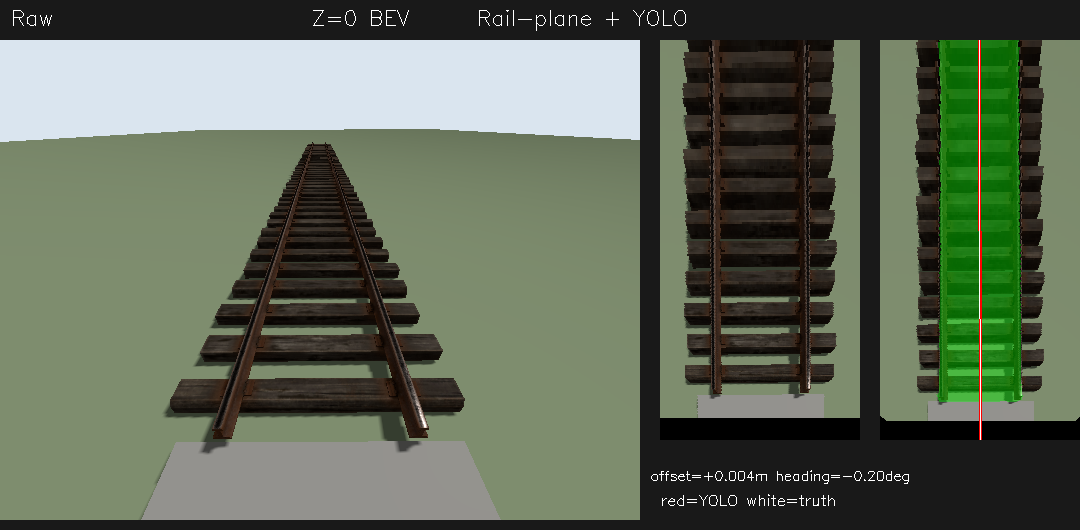
\includegraphics[width=\linewidth]{mapping-comparison.png}\caption{左：原始相机图像；中：按地面 $Z=0$ 投影；右：按轨面高度校正并叠加YOLO结果。}\end{figure}

\Needspace{12\baselineskip}\section{当前验证状态和边界}

已核对运行中的相机内参、相机与base\_link位姿，并依据GLB节点变换与SDF计算轨面高度。五帧回放完成了米制中心线与相近时刻仿真真值对照。


以下条件决定像素关系是否可信：


\begin{enumerate}
\item 单应矩阵只对目标平面成立。枕木、钢轨侧面、人员等不在同一平面上的内容会变形。
\item 图像与姿态应属于同一时刻。当前回放尚未实现曝光级同步；文件落盘时间与遥测接收时间也是近似。
\item 当前实现拒绝超过35°的roll/pitch，采用最短角插值。该软件范围不代表已完成全范围精度验证。
\item 0.02 m/像素是采样间距，不等于2 cm测量精度，远处原图可能没有足够分辨率。
\item YOLO包络不一定等于轨头中心或轨内边缘，分割宽度不能直接当标准轨距。
\item 米制中心线目前完成离线回放，还未进入飞控闭环；大横移、明显偏航与多高度测试仍待完成。
\end{enumerate}

验证顺序应是：核对内参与坐标系 → 核对高度和轨面 → 验证像素与地面往返映射 → 用独立位姿和模型尺寸评估识别结果。仅仅看到鸟瞰图中的铁轨“变直”，不足以证明尺度准确。


\end{document}
